\chapter{Antecedentes}
\section{Modelo estándar}

El modelo estándar es el formalismo teórico-experimental que hasta el día de hoy describe con mayor precisión las interacciones entre las partículas elementales y los diferentes tipos de fuerzas que experimentan las mismas. Los mayores desarrollos teóricos y descubrimientos experimentales que dieron forma al modelo estándar se tuvieron en la segunda mitad del siglo XX con el desarrollo de la Teoría Cuántica de Campo, fruto del esfuerzo de científicos de todo el mundo, los cuales a partir de los modelos teóricos y observaciones experimentales construyeron una clasificación de las partículas en base a sus propiedades fundamentales como lo son la masa, la carga eléctrica, el espín, entre otras. Dicha clasificación se muestra en la Figura \ref{fig:estandard_model}. 
\begin{figure}
    \centering
    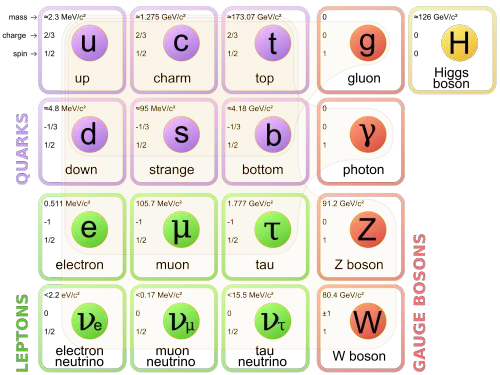
\includegraphics[width=0.84\textwidth]{ANTECEDENTES/standard_model.png}
    \caption{Clasificación de las partículas según el modelo estándar de las partículas elementales}
    \label{fig:estandard_model}
\end{figure}

Las partículas elementales están divididas en dos categorías: los fermiones y los
bosones; los fermiones están a su vez divididos en quarks y leptones los cuales tienen un valor fraccional de espín (1/2), además de que obedecen la estadística de FermiDirac y el principio de exclusión de Pauli. Los quarks son partículas elementales que constituyen a los hadrones, ya que debido al principio de confinamiento los quarks no pueden co-existir en estado libre.

Cuatro son las fuerzas fundamentales en la naturaleza: la fuerza electromagnética, la débil, la fuerte y la gravitacional. El modelo estándar incluye las tres primeras, la gravitacional no está incluida pero su contribución en la física de partículas es despreciable si se compara por ejemplo con la fuerza electromagnética (una razón de $10^{36}$ en la escala de los Giga-electrón volts). 

El modelo estándar está respaldado por una serie de observaciones experimentales, la más reciente fue la observación de una nueva partícula cuyas propiedades son consistentes con el bosón de Higgs~\cite{higgs}. Sin embargo, aún existen fenómenos en la naturaleza que no pueden ser explicados dentro del formalismo del modelo estándar, ejemplo de ello es la naturaleza y composición de la materia oscura.

\section{Materia oscura}

La materia oscura, o dark matter (por su nombre en inglés), recibe este nombre
debido a que no emite radiación electromagnética, por lo que su existencia se infiere de su influencia gravitacional sobre la materia visible (o también conocida como bariónica) que se encuentra a su alrededor; dicho fenómeno ha sido observado en cúmulos de galaxias en donde la velocidad de rotación de las mismas no corresponde a la que sería producida debido a la fuerza de gravedad ejercida por la materia visible a su alrededor.

A pesar de los esfuerzos por parte de la comunidad científica hasta este momento se desconoce la composición de la materia oscura, lo que se sabe, por medio de observaciones astronómicas, es que aproximadamente la materia oscura representa el 30.1\% de la composición materia-energía del universo, el resto es energía oscura (69.4\%) y materia visible (0.5\%). Recientemente, con el afán de entender la composición de la materia oscura y su localización en el universo, la comunidad científica ha desarrollado varios experimentos, uno de los más significativos es el Alpha Magnetic Spectrometer (AMS-02) el cual es un detector de partículas que tiene como uno de sus objetivos primordiales el de buscar indicios de materia oscura, dicho detector fue diseñado y construido en el CERN para su futura instalación en la estación espacial internacional (ISS por sus siglas en inglés). Entre sus observaciones más recientes [] se ha reportado un flujo de positrones anómalo que tiene una posible explicación en el proceso de aniquilación de partículas de materia oscura, donde se libera energía en forma de positrones. Dicho flujo anómalo puede observarse
a partir de los 25 GeV en la Figura \ref{fig:AMS_positronflux} donde también se presenta una comparación con otros experimentos que observan similar comportamiento.

\begin{figure}
    \centering
    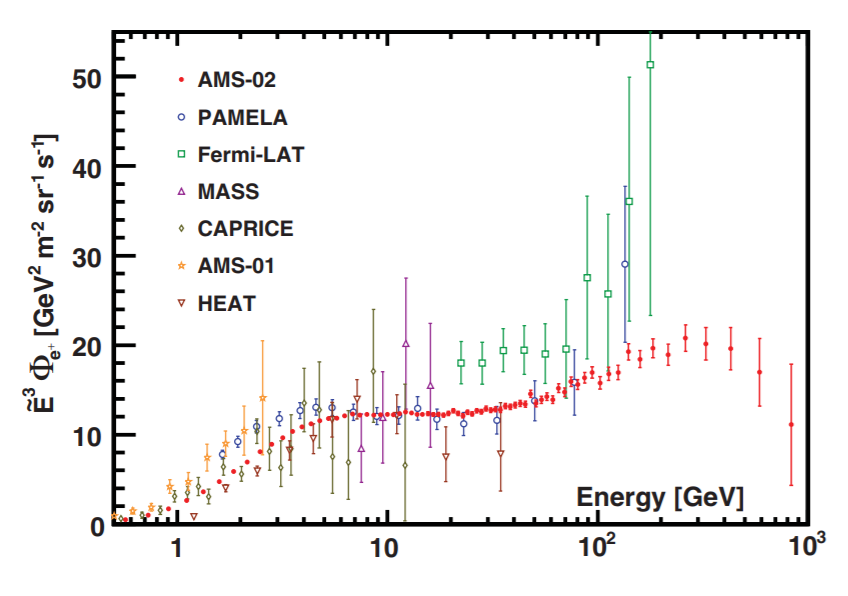
\includegraphics[width=0.84\textwidth]{ANTECEDENTES/AMS_positronflux.png}
    \caption{Flujo de positrones medido por el experimento AMS-02, comparado con los experimentos PAMELA, Fermi-LAT, MASS, CAPIRCE, AMS-01 y HEAT.}
    \label{fig:AMS_positronflux}
\end{figure}

Estas observaciones cosmológicas han motivado a los físicos teóricos de altas energías a postular nuevos modelos en los cuales la composición de la materia oscura se pueda entender por medio de nuevas partículas elementales no descritas en el modelo estándar y que sin embargo podrían estar siendo producidas en los aceleradores de partículas modernos como el Gran Colisionador de Hadrones en Ginebra, Suiza. Los modelos propuestos se encuentran en la categoría que se conoce como extensiones al modelo estándar y por lo general involucran la existencia de nuevas partículas cuyas fuerzas e interacciones están descritas por alguna variación de la teoría cuántica de campo, lo que sugiere que sus mecanismos de producción y propiedades pueden ser estudiados por el formalismo de la física de partículas y la parte experimental por medio de los detectores de partículas con métodos de recolección de datos, selección de eventos y técnicas estadísticas para el análisis y extracción de posibles señales.

\section{Experimento CMS del CERN}

El experimento considerado en este proyecto es el Compact Muon Solenoid (CMS), el cual es uno de los detectores multi-usos del CERN que tiene la capacidad de cubrir un amplio rango de procesos físicos, reportando la observación de la partícula de Higgs en el 2012. Este experimento consiste de varios subsistemas los cuales están diseñados para la identificación de prácticamente todas las partículas del modelo estándar. Para su diseño se tomó en cuenta cómo cada partícula interacciona con la materia, por ejemplo las partículas cargadas son identificadas por medio de detectores a base de silicio y de gas noble, permitiendo determinar con precisión el tiempo y localización de las partículas, así como el signo de la carga de acuerdo a la deflexión de su trayectoria debido al poderoso campo magnético solenoide de 4 Teslas que envuelve al CMS. Las partículas neutras son identificadas por la energía que depositan en los calorímetros. La variedad de interacciones por tipo de partícula se puede ver en la Figura \ref{fig:cms_interaction}

\begin{figure}
    \centering
    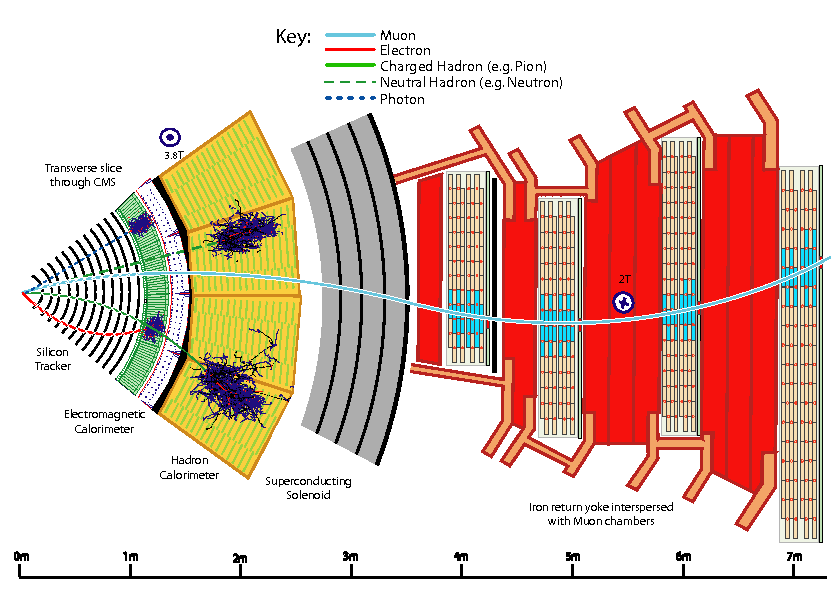
\includegraphics[width=0.84\textwidth]{ANTECEDENTES/CMS_interaction.png}
    \caption{Representación de la interacción de las partículas en el detector CMS del CERN.}
    \label{fig:cms_interaction}
\end{figure}

Los muones son partículas que interaccionan débilmente con la materia por lo que su detección se da en dos subsistemas: el detector de trazas, que corresponde a la primera capa de CMS y el sistema de muones, última capa del detector, lo cual permite una reconstrucción de trayectoria muy precisa. Debido a esto el posible decaimiento de las nuevas partículas a muones resulta en un canal favorecido desde el punto de vista experimental.



























